%%%%%%%%%%%%%%%%%%%%%%%%%%%%%%%%%%%%%%%%%
% Arsclassica Article
% LaTeX Template
% Version 1.1 (10/6/14)
%
% This template has been downloaded from:
% http://www.LaTeXTemplates.com
%
% Original author:
% Lorenzo Pantieri (http://www.lorenzopantieri.net) with extensive modifications by:
% Vel (vel@latextemplates.com)
%
% License:
% CC BY-NC-SA 3.0 (http://creativecommons.org/licenses/by-nc-sa/3.0/)
%
%%%%%%%%%%%%%%%%%%%%%%%%%%%%%%%%%%%%%%%%%

%%%%%%%%%%%%%%%%%%%%%%%%%%%%%%%%%%%%%%%%%
% Lara Olmos Camarena
% Apuntes Economía y Finanzas Matemáticas
% Curso 2016-2017
% UAM
%
% License:
% CC BY-NC-SA 3.0 (http://creativecommons.org/licenses/by-nc-sa/3.0/)
%%%%%%%%%%%%%%%%%%%%%%%%%%%%%%%%%%%%%%%%%


%--------------------------------------------------------------------------------
%	PACKAGES AND OTHER DOCUMENT CONFIGURATIONS
%--------------------------------------------------------------------------------

\documentclass[
10pt, % Main document font size
a4paper, % Paper type, use 'letterpaper' for US Letter paper
oneside, % One page layout (no page indentation)
%twoside, % Two page layout (page indentation for binding and different headers)
headinclude,footinclude, % Extra spacing for the header and footer
BCOR5mm, % Binding correction
%toc=sectionentrywithdots
]{scrartcl}

%%%%%%%%%%%%%%%%%%%%%%%%%%%%%%%%%%%%%%%%%
% Arsclassica Article
% Structure Specification File
%
% This file has been downloaded from:
% http://www.LaTeXTemplates.com
%
% Original author:
% Lorenzo Pantieri (http://www.lorenzopantieri.net) with extensive modifications by:
% Vel (vel@latextemplates.com)
%
% License:
% CC BY-NC-SA 3.0 (http://creativecommons.org/licenses/by-nc-sa/3.0/)
%
%%%%%%%%%%%%%%%%%%%%%%%%%%%%%%%%%%%%%%%%%

%----------------------------------------------------------------------------------------
%	REQUIRED PACKAGES
%----------------------------------------------------------------------------------------

\usepackage[
nochapters, % Turn off chapters since this is an article        
beramono, % Use the Bera Mono font for monospaced text (\texttt)
eulermath,% Use the Euler font for mathematics
pdfspacing, % Makes use of pdftex’ letter spacing capabilities via the microtype package
dottedtoc % Dotted lines leading to the page numbers in the table of contents
]{classicthesis} % The layout is based on the Classic Thesis style

\usepackage{arsclassica} % Modifies the Classic Thesis package

\usepackage[T1]{fontenc} % Use 8-bit encoding that has 256 glyphs

%\usepackage[utf8]{inputenc} % Required for including letters with accents
\usepackage[latin1, utf8]{inputenc}

\usepackage[spanish, activeacute]{babel}

\usepackage{graphicx} % Required for including images
\graphicspath{{Figures/}} % Set the default folder for images

\usepackage{enumitem} % Required for manipulating the whitespace between and within lists

\usepackage{subfig} % Required for creating figures with multiple parts (subfigures)

\usepackage{amsmath,amssymb,amsthm} % For including math equations, theorems, symbols, etc

\usepackage{varioref} % More descriptive referencing

\usepackage{titling}

\usepackage{multicol}
\usepackage{multirow}
\usepackage{booktabs}
\usepackage{tabularx}
\usepackage{array}
\usepackage{float}

\usepackage{cite} % para contraer referencias

\usepackage{enumitem}

\usepackage{makeidx}

%----------------------------------------------------------------------------------------
%	THEOREM STYLES
%---------------------------------------------------------------------------------------

\theoremstyle{definition} % Define theorem styles here based on the definition style (used for definitions and examples)
\newtheorem{definition}{\color{blue}{Definición}}

\theoremstyle{plain} % Define theorem styles here based on the plain style (used for theorems, lemmas, propositions)
\newtheorem{theorem}{Teorema}[section]

\theoremstyle{remark} % Define theorem styles here based on the remark style (used for remarks and notes)

%----------------------------------------------------------------------------------------
%	HYPERLINKS
%---------------------------------------------------------------------------------------
\definecolor{blue(pigment)}{rgb}{0.0, 0.28, 0.67}

\usepackage{hyperref}
\hypersetup{
%draft, % Uncomment to remove all links (useful for printing in black and white)
colorlinks=true, breaklinks=true, bookmarks=true,bookmarksnumbered,
urlcolor=blue(pigment), linkcolor=blue(pigment), citecolor=webgreen, % Link colors
pdftitle={}, % PDF title
pdfauthor={\textcopyright}, % PDF Author
pdfsubject={}, % PDF Subject
pdfkeywords={}, % PDF Keywords
pdfcreator={pdfLaTeX}, % PDF Creator
pdfproducer={LaTeX with hyperref and ClassicThesis} % PDF producer
}

%----------------------------------------------------------------------------------------
%	BACKGROUND IMAGE
%----------------------------------------------------------------------------------------

\usepackage{graphicx} \usepackage{eso-pic}

\newcommand\BackgroundPic{\put(85,50){ \parbox[b][\paperheight]{\paperwidth}{ \vfill \centering 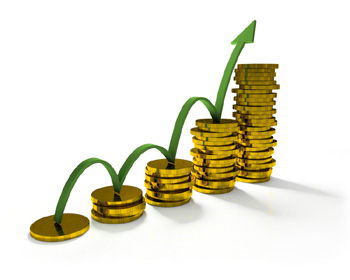
\includegraphics[width=8cm,keepaspectratio]{portada.jpg} \vfill }}}


%----------------------------------------------------------------------------------------
%	MARGIN
%----------------------------------------------------------------------------------------

\usepackage{vmargin}
\usepackage{parskip}
\setlength{\parindent}{1.5em}
\setmargins
	{3cm}		%izq
	{1.5cm}		%sup
	{15.5cm}	%anchura texto
	{22cm}		%altura texto
	{25pt}		%altura encabezados
	{1.5cm}		%espacio entre texto y encabezados
	{60pt}		%altura pie de pagina
	{1.5cm}		%espacio entre texto y pie de pagina

%----------------------------------------------------------------------------------------
%	TITLES
%----------------------------------------------------------------------------------------

%\titleformat{\section}{\textbf}{}{0cm}{}
%\titleformat{\subsection}{\textbf{\thesubsection.\thesubsectionname}}{}{0cm}{}

%----------------------------------------------------------------------------------------
%	PAGINA HORIZONTAL
%----------------------------------------------------------------------------------------

\usepackage{lscape,lipsum}

\usepackage{pdflscape}

%----------------------------------------------------------------------------------------
%	APENDICES
%----------------------------------------------------------------------------------------


%----------------------------------------------------------------------------------------
%	CUADRO COLOR
%----------------------------------------------------------------------------------------
\usepackage{framed, color}
\definecolor{shadecolor}{rgb}{0.74, 0.83, 0.9}

%----------------------------------------------------------------------------------------
%	Identacion
%----------------------------------------------------------------------------------------

\setlength{\parindent}{0pt}


%----------------------------------------------------------------------------------------
%	Encabezado y pie de pagina
%----------------------------------------------------------------------------------------

\usepackage{fancyhdr}
\usepackage{etoolbox}

%\newcommand{\fecha}{03/03/2016}

%\fancyhf{}
% \fancyhead[LO, LE]{ \begin{center}\textsc{\large{\n{\azul{PLAN DE PROYECTO}}}} \end{center} \\ Versión: {\large{\azul{\version}}} \\ Referencia: \small{\azul{\%referencia}}}

%{\footnotesize{\scshape\nouppercase{\leftmark}}}}
%\fancyhead[RO, RE]{ Página: {\large{\azul{\thepage}}} \\ Fecha: {\azul{\today}}}
% \renewcommand{\headrulewidth}{0.4pt}

%\newcommand{\headrulecolor}[1]{\patchcmd{\headrule}{\hrule}{\color{#1}\hrule}{}{}}
% \fancyfoot[LO,LE]{\vspace*{0.05cm}\includegraphics[width=2cm,height=2cm,% keepaspectratio]{logo.png}}
% 
% \fancyfoot[C]{ \\[10pt] \textsc{Soraus} \\ \textsc{Proyecto BaicUAM} }
% \fancyfoot[RO,RE]{\vspace*{0.05cm}\includegraphics[width=2cm,height=2cm,% keepaspectratio]{baicuam.jpg}}

%----------------------------------------------------------------------------------------
%	Incluir pdf
%----------------------------------------------------------------------------------------

\usepackage{pdfpages}
\usepackage{sectsty}
\sectionfont{\fontsize{17}{14}\selectfont}


%----------------------------------------------------------------------------------------
%	Nota al pie de pagina
%----------------------------------------------------------------------------------------

\renewcommand{\thefootnote}{\arabic{footnote}} 


%----------------------------------------------------------------------------------------
%	Sub sub sub seccion
%----------------------------------------------------------------------------------------

\usepackage{titlesec}

\titleclass{\subsubsubsection}{straight}[\subsection]

\newcounter{subsubsubsection}[subsubsection]
\renewcommand\thesubsubsubsection{\thesubsubsection.\arabic{subsubsubsection}}
\renewcommand\theparagraph{\thesubsubsubsection.\arabic{paragraph}} % optional; useful if paragraphs are to be numbered

\titleformat{\subsubsubsection}
  {\normalfont\normalsize\bfseries}{\thesubsubsubsection}{1em}{}
\titlespacing*{\subsubsubsection}
{0pt}{3.25ex plus 1ex minus .2ex}{1.5ex plus .2ex}

\makeatletter
\renewcommand\paragraph{\@startsection{paragraph}{5}{\z@}%
  {3.25ex \@plus1ex \@minus.2ex}%
  {-1em}%
  {\normalfont\normalsize\bfseries}}
\renewcommand\subparagraph{\@startsection{subparagraph}{6}{\parindent}%
  {3.25ex \@plus1ex \@minus .2ex}%
  {-1em}%
  {\normalfont\normalsize\bfseries}}
\def\toclevel@subsubsubsection{4}
\def\toclevel@paragraph{5}
\def\toclevel@paragraph{6}
\def\l@subsubsubsection{\@dottedtocline{4}{7em}{4em}}
\def\l@paragraph{\@dottedtocline{5}{10em}{5em}}
\def\l@subparagraph{\@dottedtocline{6}{14em}{6em}}
\makeatother

 % Include the structure.tex file which specified the document structure and layout

\hyphenation{Fortran hy-phen-ation} % Specify custom hyphenation points in words with dashes where you would like hyphenation to occur, or alternatively, don't put any dashes in a word to stop hyphenation altogether

\hypersetup{
%draft, % Uncomment to remove all links (useful for printing in black and white)
colorlinks=true, breaklinks=true, bookmarks=true,bookmarksnumbered,
urlcolor=blue(pigment), linkcolor=blue(pigment), citecolor=webgreen, % Link colors
pdftitle={Economía y finanzas matemáticas}, % PDF title
pdfauthor={Lara Olmos Camarena}, % PDF Author
pdfsubject={}, % PDF Subject
pdfkeywords={}, % PDF Keywords
pdfcreator={pdfLaTeX}, % PDF Creator
pdfproducer={LaTeX, Lara Olmos Camarena} % PDF producer
}

%---------------
% COLORES
%---------------

\definecolor{blue(pigment)}{rgb}{0.0, 0.28, 0.67}
\newcommand{\azul}{\color{blue(pigment)}}
\newcommand{\azulclaro}{\color{RoyalBlue}}

%---------------
% MACROS
%---------------

\renewcommand{\shorthandsspanish}{}
\newcommand{\n}[1]{\textbf{#1}}
\newcommand{\cur}[1]{\textit{#1}}
\newcommand{\nc}[1]{\textbf{\textit{#1}}}
	
% Colores
\newcommand{\azul}{\color{NavyBlue}}
\newcommand{\azulclaro}{\color{RoyalBlue}}
\definecolor{verde}{HTML}{008000}
\newcommand{\verde}{\color{verde}}

% Para formulas
\newcommand{\sub}[1]{_{#1}}
\newcommand{\pot}[1]{^{#1}}
\newcommand{\f}[1]{{\large{${#1}$}}}
\newcommand{\nf}[1]{\[#1\]}
\newcommand{\boldf}[1]{\f{\boldsymbol{#1}}}

\newcommand{\modulo}[1]{\parallel{#1}\parallel}
\newcommand{\integral}[4]{\int_{#1}^{#2} \! {#3} \, \mathrm{d}{#4}} 
\newcommand{\sumatorio}[2]{\sum_{#1}^{#2}} 
\newcommand{\producto}[2]{\prod_{#1}^{#2}}
\newcommand{\union}[2]{\bigcup\limits_{#1}^{#2}}
\newcommand{\interseccion}[2]{\bigcap\limits_{#1}^{#2}}
\newcommand{\sii}[0]{\Leftrightarrow}
\newcommand{\ent}[0]{\Rightarrow}
\newcommand{\menos}[0]{\smallsetminus}
\newcommand{\real}[0]{\f{\mathbb{R}} }
\newcommand{\rn}[1]{\mathbb{R}\pot{#1}}

% Contadores
\newcounter{ex}
\setcounter{ex}{1}
\newcommand{\ejemplo}{\vspace{0.4cm} {\verde{Ejemplo \arabic{ex}.}}\addtocounter{ex}{1} }

\newcounter{prop}
\setcounter{prop}{1}
\newcommand{\prop}{\vspace{0.4cm} {\n{Proposición \arabic{prop}.}}\addtocounter{prop}{1} }

\newcounter{teo}
\setcounter{teo}{1}
\newcommand{\teo}{\vspace{0.2cm} {\n{Teorema \arabic{teo}.}}\addtocounter{teo}{1} }

% Para estilos
\newcommand{\obs}[0]{{\color{purple}{\n{Observación: }}}} 
\newcommand{\dem}[0]{\verde{\n{Demostración: }}}



\makeindex


\begin{document}

%-------------------------------------------------------------------------------
%	TITLE AND AUTHOR(S)
%-------------------------------------------------------------------------------

\thispagestyle{empty}
\title{\azul{\n{\huge{Apuntes de Economía y Finanzas Matemáticas}}}}
\author{\\[200pt]\Large{Lara Olmos Camarena}} % The article author(s) - author affiliations need to be specified in the AUTHOR AFFILIATIONS block
\date{\\[200pt]\today} % An optional date to appear under the author(s)
\maketitle
\thispagestyle{empty}
\AddToShipoutPicture*{\BackgroundPic}
\ClearShipoutPicture
\vfill

\newpage

% Referencias 
\begin{thebibliography}{20}
		\bibitem{Est} Apuntes del curso de \cur{Economía y Finanzas Matemáticas II}, 2016-2017, UAM. Profesor: Rafael Orive.
		\bibitem{VicdeJuan} \cur{The Mathematics of Financial Derivatives: A Student Introduction}. Paul Wilmott, Sam Howison, Jeff Dewynne.
		\href{https://books.google.nl/books?id=HAQgAwAAQBAJ&printsec=frontcover&hl=es#v=onepage&q&f=false}{Enlace}
		\bibitem{probl} Monografías de Juan Mascareñas sobre Finanzas Corporativas (UCM).
\end{thebibliography}

\vspace{5cm}

% Advertencia y contacto
\begin{center} 
	\n{{\color{red}{¡OJO!}} Estos apuntes no están libres de errores.}
	Para cualquier corrección contactar: \href{mailto:lara.olmos@estudiante.uam.es}{lara.olmos@estudiante.uam.es}
\end{center}


%----------------------------------------------------------------------------------------
%	HEADERS
%----------------------------------------------------------------------------------------

\renewcommand{\sectionmark}[1]{\markright{\spacedlowsmallcaps{#1}}} % The header for all pages (oneside) or for even pages (twoside)
%\renewcommand{\subsectionmark}[1]{\markright{\thesubsection~#1}} % Uncomment when using the twoside option - this modifies the header on odd pages
\lehead{\mbox{\llap{\small\thepage\kern1em\color{halfgray} \vline}\color{halfgray}\hspace{0.5em}\rightmark\hfil}} % The header style

\pagestyle{scrheadings} % Enable the headers specified in this block

\newpage
\tableofcontents
%\listoffigures
\newpage


%----------------------------------------------------------------------------------------
%	CONTENIDO
%----------------------------------------------------------------------------------------


\section*{Introducción}

	\subsection*{Economía}
		El objeto de la economía es estudiar la distribución de los bienes económicos. Considera procesos de producción, comercialización, distribución y consumo para satisfacer las necesidades. Abarca estudio y análisis de:
		\begin{itemize}
			\item Forma en que se fijan los precios de bienes y factores productivos.
			\item Comportamiento mercados financieros y asignación del capital en la sociedad.
			\item Consecuencias de la intervención del Estado en la sociedad e influencia en el mercado.
			\item Distribución de la renta. Crecimiento riqueza.
			\item Influencia del gasto público, impuestos, déficit presupuestario Estado en el crecimiento estatal.
			\item Ciclos económicos, causas, oscilaciones desempleo y producción.
			\item Comercio internacional.
		\end{itemize}

	\subsection*{Finanzas}

		Rama de la economía y administración de empresas que estudia el intercambio de distintos bienes de capital entre individuos, empresas o Estados y la incertidumbre y riesgos que estas actividades conllevan.

		Estudia la \n{obtención de capital para la inversión} en bienes productivos y de las decisiones de inversión de los ahorradores. También \n{la obtención y gestión} de fondos de capital que necesita una compañía, individuo o Estado para cumplir sus objetivos, y los criterios con que dispone sus activos.

	\subsection*{Activos financieros}

		Es un instrumento financiero que otorga a su comprador el derecho a recibir ingresos futuros por parte del vendedor. Es decir, es un derecho sobre los activos reales del emisor y el efectivo que generen. 

		Un activo financiero obtiene su valor de un \n{derecho contractual}. Las monedas y billetes, por ejemplo, son títulos de deuda emitidos por el Banco Central del país.

		\subsubsection*{Características}

			\begin{itemize}
				\item \n{Rentabilidad}. Cuanto más interés aporta el activo, mayor es su rentabilidad.
				\item \n{Riesgo}. Probabilidad de que el emisor no cumpla sus compromisos. Hay riesgo de crédito, operacional y de mercado.
				\item \n{Liquidez}. Capacidad de convertir el activo en dinero sin sufrir pérdidas.
			\end{itemize}

		\subsubsection*{Activos primarios}

			Los principales o primarios son: acciones de sociedades, depósitos monetarios a plazo fijo, préstamo de una institución, bonos, pagarés, letras y obligaciones, fondos de inversión, participaciones preferentes, deuda subordinada (redimible o no, convertible en acciones).

		\subsubsection*{Clasificación según su liquidez}

			\begin{multicols}{2}
			\begin{itemize}
				\item \n{Dinero en curso legal}. Monedas y billetes.
				\item \n{Dinero en los bancos}. Depósitos a la vista, depósitos de ahorro y de plazo.
				\item \n{Deuda pública a corto plazo}. Letras del Tesoro.
				\item \n{Pagarés de empresa}. Activos emitidos por empresas privadas.
				\item \n{Deuda pública a largo plazo}. Bonos y obligaciones del Tesoro.
				\item \n{Renta fija}. Deuda emitida por las empresas privadas.
				\item \n{Renta variable}. Acciones, derivados.
			\end{itemize}
			\end{multicols}

		\subsubsection*{Derivados}

			Estos activos financieros dependen de otro activo primario, denominado \n{subyacente}. Surgen de la necesidad de eliminar el factor de riesgo de algunas actividades productivas.

			\begin{multicols}{2}
			\begin{itemize}
				\item Opciones
				\item Forwards
				\item Futuros
				\item Swaps
				\item Warrants
				\item Combinaciones
			\end{itemize}
			\end{multicols}

		\subsection*{Mercados financieros}

			Lugares, mecanismos, procedimientos donde se intercambian productos, activos o productos financieros y se fijan sus precios. 
			Existe mercados de:  
			\begin{multicols}{2}
			\begin{itemize}
				\item acciones. Bolsa.
				\item dinero.
				\item divisa.
				\item materias primas.
				\item metales preciosos.
				\item deuda pública.
				\item cuentas bancarias.
				\item derivados.
			\end{itemize}
			\end{multicols}

			Conceptos empleados:
			\begin{itemize}
				\item \n{Cartera}. Conjunto de productos adquiridos por un inversor.
				\item \n{Volatilidad}. Velocidad de cambio de los precios de los productos que se negocian.
				\item \n{Apalancamiento}. Actividad financiera en la que se utiliza el endeudamiento para financiar una inversión.
				\item \n{Especulación}. Intento de obtener ganancias por parte de un inversor a partir de su capacidad para predecir un movimiento en los precios no aticipado por el mercado.
			\end{itemize}
	\newpage

\section{Tipos de interés, préstamos y rentas}

	\subsection{Tiempo}

		Productos financieros toman el tiempo como una variable de valor añadido. Unidad fundamental: \n{año}. En muchos productos el primer día del plazo comienza a mediodía, el último termina a mediodía.

		\begin{multicols}{2}
		Reglas para contabilizar días:
		\begin{itemize}
			\item \f{30/360}, bonos mun. y corp. USA.
			\item \cur{real/real}, bonos del Tesoro en USA.
			\item \cur{real/}\f{360}, letras del Tesoro en USA.
		\end{itemize}

		\breakcolumn 

		\ejemplo \f{01/03/2017}-\f{01/09/2017}. \f{184}. 
		\begin{itemize}
			\item \f{30/360}: 6 meses, \f{180/360 = 0.5}.
			\item \cur{real/real}. \f{184/365 = 0.504}
			\item \cur{real/360}. \f{184/360 = 0.51}.
		\end{itemize}
		\end{multicols}

	\subsection{Intereses}

		Sea un préstamo de \f{K\sub{0}} de duración de t periodos. Denotamos el capital final \f{K\sub{f}} y los intereses \f{I = K\sub{f} - K\sub{0}}. Definimos:

		\begin{itemize}
			
			\item \n{Interés bruto} o rendimiento: \f{R = \frac{I}{K} = \frac{K\sub{f}-K\sub{0}}{K\sub{0}}}.
			
			\item \n{Interés simple}: \f{r\sub{s} \%}, que cumple \f{I = KR = \frac{K r\sub{s}}{100}}.

			\n{Interés simple (anual)}. \f{r\sub{s}\%}. La cantidad a devolver resulta:
			\begin{center} \f{K\sub{t} = K\sub{0} + t \frac{K\sub{0} r\sub{s}}{100}} \end{center}

			\item \n{Interés compuesto}, r por cada periodo, la cantidad a devolver es \f{K\sub{t} = K\sub{0} * (1 + r)\pot{t}}.
			El tipo equivalente para t periodos, \n{tipo compuesto}, \f{r\sub{t}}, tal que:
			\begin{center} \f{r\sub{t} = (1+r)\pot{t} - 1} = \f{\frac{I\sub{t}}{K\sub{0}}} \end{center}

			\n{Interés compuesto m veces anualmente}. La capitalización en t años es: \begin{center} \f{K\sub{t} = K\sub{0} * (1 + \frac{R\sub{m}}{m})\pot{mt}} \end{center}

			\item \n{Tipo anual equivalente}, \n{TAE}. Expresa el rendimiento actual sea cual sea su periodo. Permite comparar rendimientos de diferentes activos.
		\end{itemize}
		
		\vspace{0.3cm}
		\n{Corolario}. \f{r\sub{1}} y \f{r\sub{2}} para periodos \f{\tau\sub{1}} y \f{\tau\sub{2}}, respectivamente, son equivalentes si: \f{(1+r\sub{1})\pot{\frac{1}{\tau\sub{1}}} = (1+r\sub{2})\pot{\frac{1}{\tau\sub{2}}}}

		\ejemplo TAE de un producto con interés \f{20\%} en dos años es:
		\begin{center} \f{1 + TAE = (1 + 0,2)\pot{1/2} \ent TAE = 9,54\%} \end{center} 

		\newpage

		\ejemplo Interés compuesto m veces anualmente.
		\begin{itemize}
			\item R anual, composición trimestral: \f{TAE = (1 + R/4)\pot{4} - 1}.
			\item R anual, composición mensual: \f{TAE = (1 + R/12)\pot{12} - 1}.
			\item R semestral, composición trimestral: \f{TAE = (1 + R/2)\pot{4} - 1}.
			\item R mensual, composición diaria: \f{TAE = (1 + R/30)\pot{360} - 1}.
		\end{itemize}

		\vspace{0.3cm}

		\n{LIBOR} (London InterBank Offered Rate) es una tasa de referencia diaria basada en las tasas de interés a la cual los bancos ofrecen fondos no asegurados a otros bancos (sin riesgo) en el mercado monetario mayorista.

		\n{EURIBOR} (Euro Interbank Offered Rate) es un índice que indica el tipo de interés promedio del mercado interbancario del euro.

		\subsubsection{Tipos}

			\begin{itemize}
				\item \n{Tipo continuo}, \f{r\sub{c}}. La capitalización en t años es: \f{K\sub{t} = K\sub{0}e\pot{tr\sub{c}}}. 

				Tipo para composición anual o TAE: \f{1 + TAE = e\pot{r\sub{c}} \sii r\sub{c} = ln(1 + TAE)}

				\item \n{Tipo implícito}. \f{r\sub{1}} es el tipo hasta \f{T\sub{1}}, \f{r\sub{2}} hasta \f{T\sub{1} + T\sub{2}}. Entonces el tipo \f{r\sub{1,2}} desde el tiempo \f{T\sub{1}} hasta el \f{T\sub{1}+T\sub{2}} es: 
				\begin{center} \f{r\sub{1,2} = \frac{r\sub{2}(T\sub{1}+T\sub{2}) - r\sub{1}T\sub{1}}{T\sub{2}}} \end{center}
			\end{itemize}

	\subsection{Préstamos}

		\n{Amortizaciones de préstamos}. A la deuda inicial hay que sumar los intereses generados con un rendimiento R en cada período y restar la cantidad devuelta o cuota.
		\begin{center} \f{I\sub{t} = K\sub{t-1} * R} \\ \f{K\sub{t} = K\sub{t-1} + I\sub{t} - C\sub{t}} \end{center}

		Suponemos que la cuota de amortización es constante (sistema de amortización francés). La cuota C que anula el capital en la amortización es, dado N en años:
		\begin{center} \f{C = \frac{RK\sub{0}}{1 - (1 + R)\pot{-N}}} \end{center}

		Dado interés anual R, con composición y amortización \n{mensual}:
		\begin{itemize}
			\item El interés anual R se sustituye por interés mensual: \f{R/12}.
			\item El contador de períodos se mide en meses, de N años a \f{12*}N meses.
		\end{itemize}
		\begin{center} \f{C = \frac{K\sub{0} * R/12}{1 - (1 + R/12)\pot{-12N}}} \end{center}

	\subsection{Valorar inversiones}

		Queremos determinar el valor a partir de los pagos y costes en fechas futuras dependiendo de unos intereses.

		\begin{itemize} 
			\item \n{Valor actual} de un pago C que tendrá lugar en una fecha futura, \n{t años}, con \n{R el tipo libre de riesgo anual} para el vencimiento.
			\begin{center} \f{VA = \frac{C}{(1+R)\pot{t}} = PV} (present value) \end{center}

			\item Dados unos flujos \f{F\sub{1},...,F\sub{n}} en las fechas \f{t\sub{1},...,t\sub{n}} en años, el valor actual es:
			\begin{center} \f{PV = \sumatorio{i=1}{n} \frac{F\sub{i}}{(1+R)\pot{t\sub{i}}}} \end{center}

			\item Sea \f{C\sub{0}} el coste inicial de la inversión. El \n{valor neto actual} es \f{NPV = PV - C\sub{0}}.
		\end{itemize}

		Sea una inversión inicial \f{C\sub{0}} y unos flujos \f{F\sub{1},...,F\sub{n}} en las fechas \f{t\sub{1},...,t\sub{n}}. La \n{tasa interna de rendimiento} o \f{TIR} al tipo \f{R\pot{*}} que anula el valor neto actual, es: 
		\begin{center} \f{\sumatorio{i=1}{n} \frac{F\sub{i}}{(1+R\pot{*})\pot{t\sub{i}}} = C\sub{0}} \end{center}

		Sea una inversión inicial P que da lugar a unos ingresos E hasta T. Definimos:
		\begin{itemize}
			\item \n{Rendimiento bruto} o \n{ROI}\f{= E/P}. Si es un activo variable, \f{P = P\sub{0}} y el precio inicial \\ \f{E = P\sub{T} - P\sub{0} + I}, donde \f{P\sub{T}} es el precio final e I son los ingresos o dividendos aportados.
			\item \n{Tiempo de retorno} o \n{TOR}\f{= 1/ROI}.
			\item \n{Razón precio-beneficio} o \n{PER} de una acción al cociente. \f{PER = P/BPA}, donde P es el precio por el que se adquiere o cotiza la acción y BPA es el beneficio por acción, el dividendo de cada acción después de impuestos.
		\end{itemize}

	\subsection{Bonos}

		Un \n{bono} es un título de deuda, definido por los parámetros: nominal (N), vencimiento (T), cupones \f{C\sub{i}} a pagar en fechas \f{t\sub{i}} (\n{t expresado en años}).

		Dado un bono de precio P, la \n{TIR del bono} (rendimiento o interés) cumple:
		\begin{center} \f{P = \frac{N}{(1+TIR)\pot{T}} + \sumatorio{i = 1}{T} \frac{C\sub{i}}{(1 + TIR)\pot{t\sub{i}}} } \end{center}

		Modelo \n{interés continuo}:
		\begin{center} \f{P = \sumatorio{t = 1}{T-1} C\sub{i} e\pot{-yt} + (C\sub{T} + N)e\pot{-yT}} \end{center}

		\subsubsection{Bono cupón cero}
		
		Título que no paga cupones ni intereses durante su vida, lo hace íntegramente en el momento en el que se amortiza (cuando el importe del bono es devuelto).

		\begin{center}\f{VA = \frac{N}{(1+r)\pot{t}}} \hspace{0.5cm} \f{P = \frac{N}{(1+r)\pot{t}}} \hspace{0.5cm} (\f{r = TIR}) \end{center} 
				
		Rendimiento de un bono cupón cero se obtiene (de precio P, nominal N y TIR \f{r\sub{T}}): \f{P = \frac{N}{(1+r\sub{T})\pot{T}}}
		
		\subsubsection{Bono a la par}

		Dado un determinado vencimiento, el \n{rendimiento a la par} es la tasa de cupón que igualaría el precio del bono con su valor nominal. Llamamos \n{bono a la par}, aquel cuya tasa cupón viene dada por el rendimiento a la par.

		\subsubsection{Curvas de interés}

			La estructura temporal de los tipos de interés (ETTI), o curvas de rendimientos, representa la relación existente en un momento dado entre el rendimiento de un conjunto de bonos (con el mismo riesgo) y el tiempo que resta hasta el vencimiento.

			Se representa mediante una sucesión de puntos y su interpolación donde cada punto muestra el interés a un periodo fijo hasta su vencimiento y el plazo de tiempo hasta el mismo. 

			Tenemos tres tipos de curvas: rentabilidad a vencimiento o TIR (\n{curva de rentabilidad}), contado o spot (\n{curva cupón cero}) o a plazos implícitos o forward.
			
			\subsubsubsection{Curva cupón cero}

				El valor de cualquier activo (bonos en este caso) viene dado por el valor actual de los flujos de caja que promete generar a lo largo de su vida. Se puede contemplar también como una cartera de valores formada por tantos bonos cupón-cero como cupones prometa generar.

				Para obtener el valor actual del activo basta conocer el valor de los cupones cero en que se descompone, y con ellos obtener los \cur{tipos al contado} de la \n{curva de rendimientos cupón-cero}.

				Las curvas de cupón cero de valores \f{(R\sub{1}, R\sub{2},...)} para las anualidades \f{1,2,...}, facilitan la obtención del precio de un bono de anualidades de nominal N y de cupones \f{C\sub{i}}.
			\begin{center} \f{P\sub{n} = \frac{C\sub{n} + N}{(1+R\sub{n})\pot{n}} + \sumatorio{i=1}{n-1} \frac{C\sub{i}}{(1+R\sub{i})\pot{i}}} \end{center}


				\ejemplo

				\begin{multicols}{2}
				\begin{tabular}{|c|c|c|c|c|}
				\hline
				Bono & 0 & 1 & 2 & 3\\
				\hline
				A & 111,41 & 10 & 110 & 0\\
				B & 102,82 & 5 & 5 & 105\\
				C & 88,9 & 0 & 0 & 100\\
				\hline
				\end{tabular}

				\breakcolumn

				\f{ \left\{ 
				\begin{aligned}
				111,41 &= 10 x + 110 y \\ 
				102,82 &= 5x+5y+105z \\ 
				88,9 &= 100z
				\end{aligned}}
				\end{multicols}

				Con \f{x = \frac{1}{1+r\sub{1}}}, \f{y = \frac{1}{(1+r\sub{2})\pot{2}}} y \f{z = \frac{1}{(1+r\sub{3})\pot{3}}}

			\subsubsubsection{Curva tiempo implícito}

				La fórmula que nos da el interés a plazo implícito a un año a partir de la curva cupón cero es:
				\begin{center} \f{R\sub{i,i+1}} = \f{R\sub{i,1}} = \f{\frac{(1 + R\sub{i+1})\pot{i+1}}{(1+R\sub{i})\pot{i}} - 1} \end{center}

				Si la curva es plana, los intereses no varían en el futuro, si crece/decrece tipos anuales más altos/bajos.

		\newpage

		\subsubsection{Duración}

			Es una media ponderada de los vencimientos de los pagos por el valor actual relativo de los mismos.

			\begin{center}
			\vspace{0.3cm}
			\begin{tabular}{|c|c|c|}
			\hline
			Tipo de interés & Precio & Duración\\
			\hline
			Continuo & \f{P = \sumatorio{i = 1}{n} c\sub{i}e\pot{-rt\sub{i}} + Ne\pot{-rt\sub{n}}} & \f{D = \frac{1}{P} \sumatorio{i=1}{n} t\sub{i}c\sub{i}e\pot{-rt\sub{i}}} + N t\sub{n} e\pot{-rt\sub{n}}}  \\
			\hline
			Compuesto & \f{P = \sumatorio{i=1}{n} \frac{c\sub{i}}{(1+R)\pot{t\sub{i}}} + \frac{N}{(1+R)\pot{t\sub{n}}}} & \f{D = \sumatorio{i=1}{n} \frac{t\sub{i}c\sub{i}}{P(1+R)\pot{t\sub{i}}} + \frac{N}{P(1+R)\pot{t\sub{n}}}} \\
			\hline
			\end{tabular}
			\end{center}

			\vspace{0.3cm}

			\n{Observación}. La duración de un bono cambia a lo largo de su vida. Para un bono cupón cero no.

			La duración mide la vulnerabilidad a cambios de los intereses. Para tipo continuo:
			\begin{center} \f{D = \frac{-1}{P} \frac{dP}{dr}} \end{center}

			\subsubsubsection{Sensibilidad}
				
				Derivada del precio del bono con respecto a cambios en la TIR. Resulta: \begin{center} \f{\Delta P = -DP\Delta r} \end{center}


	\newpage

\section{Derivados}

	\subsection{Swaps}

		Un \n{swap} es un contrato entre dos partes que intercambian intereses sobre un cierto nominal hasta un cierto plazo: una parte paga intereses con un \n{tipo fijo}, la otra parte paga intereses según un tipo \n{variable} (Euríbor). En principio, \n{no hay intercambio de nominales}.
		No se negocia en mercados regulados. Tipos:
		\begin{itemize}
			\item Tipo de intereses (fijo o variable).
			\item Divisas
			\item Renta variable (equity swap)
		\end{itemize}

		\subsubsection{Swap de tipo de interés}

			Transforma los tipos de interés para mejorar las ofertas recibidas de tipos o reducir el riesgo de las operaciones. Puede ser fijo o variable (flotante).

			Tienen como parámetros: \n{nominal} (N), \n{fechas} (\f{t\sub{1},...,t\sub{n}}), tipo de interés (R para fijo, LIBOR para variable).

			\subsubsubsection{Valoración}

				Depende en signo de a quien va dirigido. \n{Consideremos el caso de quien paga interés fijo y recibe el flotante}:
				\begin{center} \f{V\sub{swap} = B\sub{fl} - B\sub{fix}} \\ \f{B\sub{fix} = \sumatorio{i=1}{n} ke\pot{-r\sub{i}t\sub{i}} + Ne\pot{-r\sub{n}t\sub{n}}} \\ \f{B\sub{fl} = (k\pot{*} + N) e\pot{-r\sub{1}t\sub{1}}} \end{center}

				donde k es el pago de tipo fijo, \f{k\pot{*}} es el pago de tipo flotante y \f{r\sub{i}} son los tipos de interés relevantes a los vencimientos \f{t\sub{i}}.

				Si un \n{swap} se firma en la media de las cotizaciones de oferta y demanda tendrá \n{valor \f{0}}, es decir, \f{B\sub{fl} = B\sub{fix}} y:
				\begin{center} \f{B\sub{fix} = \sumatorio{i=1}{n} ke\pot{-r\sub{i}t\sub{i}} + Ne\pot{-r\sub{n}t\sub{n}}} \\ \f{B\sub{fl} = (k\pot{*} + N) e\pot{-r\sub{1}t\sub{1}} = N} \end{center}

				siendo \f{y\sub{n}} el tipo TIR asociado a la curva cupón cero de tipos continuos \f{r\sub{1},...,r\sb{n}}: 
				\begin{center} \f{k = N (e\pot{y\sub{n}t\sub{1} - 1})} \end{center}

				El tipo fijo del swap sería el \f{TIR\sub{n}} si lo consideramos como interés compuesto anual. 

				Al vencimiento es cero.

		\subsubsection{Swap de divisas}

			Implica intercambios de pagos de principal e intereses de tipo fijo o flotante sobre un préstamo en una divisa, por pagos de principal e intereses de tipo fijo o flotante sobre otro préstamo en otra divisa.

			Parámetros: \f{N\sub{1},N\sub{2}} nominales, \f{t\sub{1},...,t\sub{n}} fechas, \f{R\sub{1}, R\sub{2}} tipos de interés (fijos) para cada divisa.

			\subsubsubsection{Valoración}

				Depende en signo de a quien va dirigido. \n{Consideremos el caso de quien paga interés fijo y recibe el flotante}:
				\begin{center} \f{V\sub{swap}(t) = B\sub{1}(t) - X\sub{1/2}(t)B\sub{2}(t)} \end{center}

				donde \f{B\sub{i}} es el valor de la divisa \f{i}, \f{X\sub{1/2}} es el valor del cambio de la divisa \f{1} con respecto a la \f{2}.

				El valor inicial de un swap de divisas no tiene por qué ser \f{0}.

	\subsection{Arbitraje}

		Es la práctica de obtener ventaja de una diferencia de precio entre dos o más mercados: realizar una combinación de transacciones complementarias que capitalizan el desequilibrio de precios. La utilidad se logra debido a la diferencia de precios de los mercados.

		Ante una posibilidad de arbitraje se producen una combinación de transacciones complementarias que resulta el equilibrio de mercado.

		Si los precios de mercado no permiten la ejecución de arbitraje rentable, entonces los precios están en \n{equilibrio de arbitraje} o el mercado es \n{libre de arbitraje}.

	\subsection{Contrato a plazos (forward)}

		Es un acuerdo privado para intercambiar un activo por dinero (u otro activo) en una fecha futura determinada. En él participa:
		\begin{itemize}
			\item \n{Posición larga}, quien \n{compra} el activo. A tiempo T paga \f{F\sub{0}} por el producto financiero.
			\item \n{Posición corta}, quien \n{vende} el activo. A tiempo T recibe \f{F\sub{0}} por el producto financiero que entrega.
		\end{itemize}

		Parámetros: 
		\begin{multicols}{2}
		\begin{itemize}
			\item \f{T} tiempo de la firma del contrato hasta finalización, 
			\item \f{S\sub{t}} valor del subyacente en \f{t \in [0,T]}, 
			\item \f{F\sub{t}} el precio a plazo en t que vence en T
			\item \f{r = r(t,T)} el tipo continuo libre de riesgo
		\end{itemize}
		\end{multicols}

		No se negocian en mercados. Es vinculante. Se liquida por entrega o diferencia. Se \n{fija el precio del activo en el contrato}. Los flujos finales son funciones lineales del subyacente. Se usa en coberturas, especulación. 

		Se establecen de tal forma que su valor inicial sea cero, no cuesta nada tener posición corta o larga.

		El precio actual de un forward es el precio de entrega que se aplicaría si el contrato se negociara hoy. El precio de entrega es el precio a plazo de cuando se firma.

		\vspace{0.2cm}

		\begin{framed}
		\n{Teorema}. Supongamos precios en equilibrio de arbitraje. Entonces el precio de la entrega en T de una unidad de subyacente es: \f{F\sub{0} = S\sub{0}e\pot{rT}}

		\n{Con dividendos conocidos}. El subyacente paga dividendos cuyo valor actual es \f{D\sub{0}}. Entonces:
		\begin{center} \f{F\sub{0} = (S\sub{0}-D\sub{0})e\pot{rT}} \end{center}

		\n{Rendimiento anual medio}, q. Entonces: \f{F\sub{0} = S\sub{0}e\pot{(r-q)T}} 
		\end{framed}


		\subsubsection{Valoración dinámica de un contrato}

			Refleja la diferencia entre lo que se contrató y el valor de hacer el contrato en ese momento. Es decir, queremos calcular el valor de un contrato \f{f\sub{t}} en el tiempo \f{t \in (0,T)} para un contrato realizado en \f{0} y que finaliza en \f{T}.

			En \f{t = 0} \f{\ent} \f{f\sub{0} = 0}
			En t: \f{f\sub{t} = (F\sub{t}-F\sub{0})e\pot{-r(T-t)} = S\sub{t}-F\sub{0}e\pot{-r(T-t)}}

			En el caso de dividendos o rendimientos conocidos: \\
			\f{f\sub{t} = S\sub{t}-I\sub{t}-F\sub{0}e\pot{-r(T-t)}} \hspace{0.3cm} o \hspace{0.3cm} \f{f\sub{t} = S\sub{t}e\pot{-q(T-t)}-F\sub{0}e\pot{-r(T-t)}} \\
			donde \f{I\sub{t}} es el valor actual de los ingresos o q es el rendimiento anual medio.

		\subsubsection{Valoración neutral de riesgo}

			Cualquier activo dependiente de otros activos puede valorarse sobre el supuesto de que los inversores son neutrales al riesgo. Se mantienen dos resultados:
			\begin{enumerate}
				\item La rentabilidad esperada en todos los activos es el tipo de interés libre de riesgo.
				\item El tipo de interés libre de riesgo es el tipo de descuento apropiado a aplicar a cualquier futuro flujo de caja
			\end{enumerate}

		\subsubsection{Vender a corto}

			Es una estrategia de arbitraje o especulación. Implica vender activos que no se tienen. 

			\ejemplo
			\begin{enumerate}
				\item Inversor I vende a corto \f{500} acciones. Su agente A toma prestadas \f{500} acciones y las vende en el mercado.
				\item I mantiene la posición mientras pueda.
				\item I liquida la posición comprando \f{500} acciones. A devuelve el préstamo.
			\end{enumerate}

			Conclusión: si baja la acción hay beneficios. Si sube, pérdidas. El agente exige una garantía o depósito inicial a los clientes a corto.


		\newpage

	\subsection{Futuros}

		Es un acuerdo entre dos partes para comprar o vender un activo en una fecha futura y a un precio previamente pactado (se pacta en el presente pero se liquida en el futuro). Su origen es la necesidad de cubrir el mercado de materias primas ante riesgos (cobertura).

		A diferencia de los \cur{forward}, los contratos de futuros son estandarizados y se operan en un mercado organizado o bolsa de productos derivados (las dos partes no se conocen necesariamente). Se ajusta diariamente en el mercado.

		Fijan la cantidad, calidad del subyacente, último día de negociación y la entrega.

		Si el activo es objeto de inversión para inversores (futuros sobre índices, divisas, oro y plata) el precio a plazo de un futuro y su valoración es igual que en un \cur{forward} siempre que el interés sea constante o función conocida en el tiempo.

		\subsubsection{Coste de almacenamiento}

			El valor del contrato se incrementa: \f{K = F\sub{0} = (S\sub{0} + U\sub{0}) e\pot{rT}}, \f{F\sub{0} = S\sub{0} e\pot{(r+u)T}}, donde \f{U\sub{0}} es el valor actual del coste de almacenamiento (o de una proporción u del producto).

		\subsubsection{Arbitraje en futuros}

			\begin{itemize} 
				\item Caso \f{F\sub{0} > (S\sub{0} + U)e\pot{rT}}. 
				\begin{enumerate}
					\item Pedir un préstamo por \f{S\sub{0}+U}.
					\item Compramos el activo y pagamos el almacenaje.
					\item Ponernos a corto. Vendemos un futuro a precio de entrega \f{F\sub{0}}.
					\item En \f{t = T} entregamos el futuro y recibimos \f{F\sub{0}}. 
					\item Pagamos el préstamo.
					\item \n{Beneficio final}: \f{F\sub{0} - (S\sub{0}+U\sub{0}) e\pot{rT}}.
				\end{enumerate}

				\item Caso \f{F\sub{0} < (S\sub{0}+U)e\pot{rT}}.
				\begin{enumerate}
					\item Tenemos el producto \f{S\sub{0}} almacenado.
					\item Vendemos el producto \f{S\sub{0}} y el almacenamiento.
					\item Posición larga, compramos un futuro \f{F\sub{0}}.
					\item \n{Beneficio final}: \f{(S\sub{0} + V\sub{0}) e\pot{rT} - F\sub{0}}.
				\end{enumerate}
			\end{itemize}

		\subsubsection{Tasa de conveniencia}

			El disponer de la mercancía presenta ventajas a quien la mantiene y produce descuento en el precio de entrega. Estos beneficios son \n{rendimientos de conveniencia}, \f{y}:
			\begin{center} \f{F\sub{0}e\pot{yT} = (S\sub{0}+U\sub{0})e\pot{rT}}, \hspace{0.3cm} \f{F\sub{0} = S\sub{0}e\pot{(r+u-y)T}} \end{center}
			Refleja las expectativas del mercado concernientes a la disponibilidad futura del producto.

		\subsubsection{Coste de mantenimiento}

			Mide el coste de almacenamiento más el interés que se paga para financiar el activo y menos el ingreso generado por el mismo. Definido como \f{c}:
			\begin{center} \f{F = Se\pot{cT}} (activo de inversión), \hspace{0.3cm} \f{F = Se\pot{(c-y)T}} (de consumo) \end{center}
			(\f{y} es la tasa de conveniencia)

		\subsubsection{Futuros sobre bonos del Tesoro (CBOT)}

			Puede ser entregado:
			\begin{itemize}
				\item Bono del estado con más de \f{10} años para su vencimiento.
				\item Sin amortización anticipada antes de \f{10} años.
				\item Hay futuros para vencimientos de \f{2}, \f{5} años.
			\end{itemize}

			Los precios se cotizan en dólares y treintaidosavos de dólar. Precio de la cotización de un bono es:\\
			\cur{P. bono en metálico = P. cotización B + Interés devengado}

			Para la posición \n{corta} se ha de determinar: el \n{factor de conversión} (\f{f\sub{c}}) para definir el precio y el bono a entregar (el más barato).

			\cur{A recibir p.c. = Cotización F * \f{f\sub{c}} + Interés acumulado}

			\subsubsubsection{Factor de conversión bono}

				\begin{itemize}
					\item Es igual al precio del bono al primer día del mes de entrega.
					\item a un TIR anual compuesto semestral.
					\item Vencimiento y pagos de cupón en trimestres por defecto.
				\end{itemize}

		\subsubsection{Precio de cotización de un futuro}
			\begin{enumerate}
				\item Determinar que una obligación aceptada sea la más barata.
				\item Calcular factor de conversión de la obligación.
				\item Calcular precio en efectivo del bono, S.
				\item Calcular el precio del futuro \f{F = (S-I)e\pot{rT}}, donde I es el valor actual de los cupones a pagar antes de la entrega.
				\item Calcular la cotización del futuro a partir de la tesorería de la posición corta.
			\end{enumerate}

			\begin{center} \f{Cotización(F) = \frac{F - Interés acumulado}{f\sub{c}}} \end{center}

		\subsubsubsection{Coberturas con futuros}

			\begin{itemize}
				\item \n{Cobertura corta}. Tiene un producto o sabe que lo va a tener. Se quiere compensar una posición larga (venta futuro).
				\item \n{Cobertura larga}. Va a necesitar el producto. Compensar una posición corta. (Pueden usarse opciones).
			\end{itemize}

			\n{Observación}: no tienen por qué ser los mismos activos subyacentes. A lo mejor no se conoce la fecha, previo a la liquidación. Consecuencia: \n{Riesgo de base}.
			\begin{center} \cur{Base = Precio de contado activo cubierto - Precio del futuro utilizado} \end{center}


		\subsubsubsection{Ratio de cobertura}

			Es el cociente entre el tamaño de la posición tomada en contratos de futuros sobre el tamaño del activo expuesto.
			\begin{itemize}
				\item \f{\Delta S}. Cambio en el precio de contado, S.
				\item \f{\Delta F}. Cambio en el precio del futuro, F.
				\item \f{\sigma\sub{S}}. Desviación estándar de \f{\Delta S}. 
				\item \f{\sigma\sub{F}}. Desviación estándar de \f{\Delta F}.
				\item \f{\rho}. Coeficiente de correlación entre \f{\Delta S} y \f{\Delta F}.
			\end{itemize}

			\n{Recordatorio}: \f{\sigma\sub{x} = \frac{1}{n-1} \sumatorio{i=1}{n} (x\sub{i}-\bar{x})\pot{2}}.

			El \n{ratio de cobertura de varianza mínima}, \f{h\pot{*}} es:
			\begin{center} \f{Var(\Delta S - h\pot{*}\Delta F) = min\{Var(\Delta S - h\Delta F), h\in \rn{+}\}} \end{center}

			Minimiza el riesgo de la cartera resultante de la cobertura, 
			\begin{center} \f{h\pot{*} = \rho \frac{\sigma\sub{S}}{\sigma\sub{F}}} \end{center}

			\vspace{0.3cm}
			
			\begin{framed}
			\n{Número óptimo de contratos de futuros para cubrir un activo A}.
			\begin{itemize}
				\item \f{N\sub{A}}. Número de unidades de A que esperamos vender en el tiempo T.
				\item \f{N\sub{F}}. Número de unidades de A que contratamos como futuro a T.
				\item \f{Q\sub{F}}. Tamaño en unidades del contrato de futuro F. 
			\end{itemize}

			Entonces el ratio de cobertura es:
					\begin{center} \f{h\pot{*} = \frac{N\sub{F}}{N\sub{A}}} \end{center}
			y el \n{número óptimo de contratos de futuros}, \f{N\pot{*}} es:
				\begin{center} \f{N\pot{*} = \frac{N\sub{F}}{Q\sub{F}} = h\pot{*}\frac{N\sub{A}}{Q\sub{F}}} \end{center}
			\end{framed}


		\subsubsection{Futuros sobre índices}


			Precio de entrega viene dado: \f{F = Se\pot{(r-q)T}} donde r es el tipo libre de riesgo y q es la tasa continua de rendimientos por dividendos. También se puede obtener a partir de la cantidad de dividendos D. \begin{center} \f{F = (S-D)e\pot{rT}} \end{center}

			Hacer cobertura sobre una cartera de acciones del índice:

			Sea P el precio de la cartera de acciones que vamos a cubrir, M el valor del índice del mercado, A el valor actual de las acciones subyacentes al índice, \f{N\pot{*}} el número de futuros de índice de mercado.

			Entonces \f{N\pot{*} = \beta \frac{P}{A}} donde el parámetro \f{\beta} es: \f{\beta = \frac{cov(P,M)}{\sigma\pot{2}\sub{M}}}

			\f{\beta} nos da la relación entre la rentabilidad de la cartera de acciones P y la rentabilidad del mercado según el modelo de variación de activos financieros.

		\subsubsection{Futuro sobre bono}

			Dado el tipo libre de riesgo r (suponemos constante) y \f{t\sub{1},...,t\sub{n}} pasos de los cupones. El precio del bono es:
			\begin{center}\f{P = \sumatorio{i}{} c\sub{i}e\pot{-r\sub{i}t\sub{i}} + Ne\pot{-r\sub{n}t\sub{n}}}\end{center}

			\f{D = \frac{-1}{P} \frac{dP}{dr}} \f{\ent} \f{\Delta P = -DP \Delta r}

			Dados dos bonos con sus duraciones \f{D\sub{1},D\sub{2}} y sus precios \f{a\sub{1},a\sub{2}}, tenemos:\\
			\f{D = \frac{a\sub{1}}{a\sub{1}+a\sub{2}}D\sub{1} + \frac{a\sub{2}}{a\sub{1}+a\sub{2}}D\sub{2}}

			\f{\Delta F = -D\sub{F} F \Delta r}

		\subsubsection{Coberturas y duración}

			Sea F el precio del contrato de futuros, \f{D\sub{F}} la duración del subyacente al futuro, \f{P} el precio actual de la cartera, \f{D\sub{P}} duración de la cartera al vencimiento de la cobertura.

			El número de contratos de futuros para cubrirse frente a un movimiento paralelo de la curva de interés es:
			\begin{center} \f{N\pot{*} = \frac{PD\sub{P}}{FD\sub{F}}} \end{center}

		\newpage

	\subsection{Opciones}

		Contrato que permite vender o adquirir un subyacente a un precio prefijado en un momento determinado (\n{opción europea}) o hasta un momento dado (\n{opción americana}). 
		\begin{itemize}
			\item El momento dado es la \n{fecha de vencimiento} (T).
			\item Para suscribir el contrato de opciones se debe pagar un \n{precio de adquisición} de la opción.
			\item El precio prescrito del subyacente es el \n{precio de ejercicio}, \n{strike} o de cierre.
			\item \n{Valor intrínseco} de una opción es el máximo entre 0 y el valor que tendría si fuera ejercida en ese momento.
		\end{itemize}

		Tienen dos usos: especulación y cobertura. Se pueden realizar opciones con subyacentes como divisas, futuros, índices, acciones. Hay distintas posiciones:
		\begin{itemize}
			\item Posiciones \n{largas}. \n{Compradores de opciones} de compra o de venta.
			\item Posiciones \n{cortas}. \n{Vendedores de opciones} de compra o de venta.
		\end{itemize}

		El emisor (\cur{writer} o vendedor) de la opción y el comprador (o \cur{holder}) tienen como intermediarios la \cur{Cámara de Compensación} (\cur{clearing house}), los \cur{brokers} y creadores de mercado (\cur{market makers}).
		\vspace{-0.3cm}

		\subsubsection{Tipos de opciones}
		\begin{itemize}
			\item \n{Opción de compra (call)} da a su propietario el \n{derecho a comprar} un activo a cierto precio. La otra parte tiene obligación de vender el subyacente si se ejerce el derecho. %es pagado en el momento de apertura del contrato.
			\item \n{Opción de venta (put)} da a su propietario el \n{derecho a vender} un activo a un cierto precio. Obliga a la otra parte a comprar el subyacente si se ejerce el derecho.
		\end{itemize}

		\cur{Observación}: Derecho para el comprador de la opción, obligación para el emisor de la opción. El comprador de una opción, para asegurarse que el vendedor puede entregarle el subyacente, exige (a través de intermediarios) que el vendedor proporcione una \n{garantía} (por ejemplo depósito de x\% del valor de mercado del título).

		\vspace{-0.3cm}

		\subsubsection{Posibilidades para el comprador de la opción (europea)}

		\begin{enumerate}
			\item Ejercer el derecho comprando o vendiendo los títulos que la opción le permite.
			\item Dejar pasar la fecha de vencimiento sin ejercer su opción.
			\item Venderla antes de su vencimiento en el mercado secundario de opciones.
		\end{enumerate}

		\ejemplo A fecha de 28 de abril, firmamos la opción de compra para el 28 de octubre para comprar un subyacente a precio de ejercicio de 250 euros. El coste de la opción de compra es 10 euros. Hay dos posibles situaciones dadas por el precio del subyacente en la fecha de expiración (28 de octubre).
		\begin{enumerate}
			\item Si el precio del subyacente es 270 euros el 28 de octubre, podremos comprar el subyacente solo por 250 euros. Obtenemos un beneficio de 10 euros porque podemos revenderlo inmediatamente en el mercado a 270 euros (hay que restar el precio de la opción).
			\item Si el precio del subyacente es 230 euros el 28 de octubre, entonces, ¿para qué comprar a 250 euros, estando en el mercado a 230?
		\end{enumerate}

		\subsubsection{Opciones sobre acciones}
		
			Los factores que determinan los precios de las opciones sobre acciones (europea, americana) de compra (c, C) o venta (p, P) son: el \n{precio actual de las acciones} S, \n{precio de ejercicio} X, tiempo de expiración T, volatilidad del precio de las acciones \f{\sigma}, el \n{tipo libre de riesgo} r, \n{dividendos} esperados durante la vida de la opción, de valor actual D. Los precios de las opciones tienen un límite máximo y mínimo, sino hay oportunidades de arbitraje.

			\vspace{-0.4cm}

			\subsubsubsection{Opción de compra}

			\n{La opción no puede tener más valor que la acción:} \f{c,C \leq S}. \\Sobre las acciones que \n{no distribuyen dividendos} se satisface: \f{c \geq max(S-Xe\pot{-rT}, 0)}


			\begin{itemize}
				\item \n{Punto de vista del comprador}. Paga el precio de adquisición de la opción. Al adquirir una opción de compra, se puede beneficiar de un aumento en el precio del activo subyacente sin haberlo comprado. El poseedor de la opción de compra sobre una acción (tiene posición larga en opciones de compra, pero posición corta en las acciones porque no las tiene) puede decidir si ejercer o no la opción, dependerá del precio de cotización de la acción.

				\item \n{Punto de vista del vendedor}. Recibe el precio de adquisición de la opción. Si el precio de cotización de la acción asciende, al tener la obligación de vender la acción tendrá pérdidas.
			
			\end{itemize}
				
					\begin{figure}[h!]
						\begin{multicols}{2}
						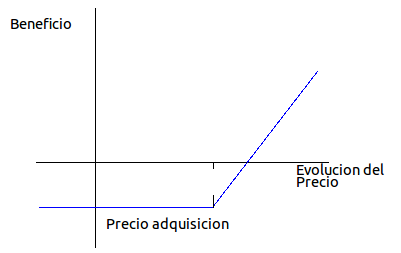
\includegraphics[width=5cm, keepaspectratio]{opcioncompracomprador.png}
						\caption{Punto de vista del comprador en t = T}

						\breakcolumn
						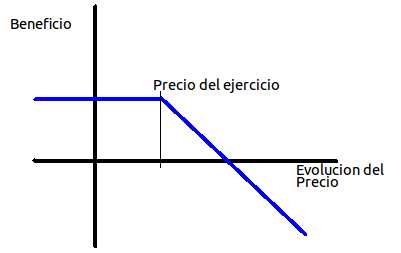
\includegraphics[width=5cm, keepaspectratio]{opcioncompravendedor.png}
						\caption{Punto de vista del vendedor en t = T}
						\end{multicols}
					\end{figure}

			\vspace{-0.7cm}

			\subsubsubsection{Opción de venta}

			\n{La opción de venta no puede tener más valor que el strike:} \f{p,P \leq X}. \\En la opción europea a vender en T, \f{p \leq Xe\pot{-rT}}. \\La opción europea sobre acciones que \n{no distribuyen dividendos} satisface: \f{p \geq max(Xe\pot{-rT} - S, 0)}

				\begin{figure}[h!]
					\begin{multicols}{2}
					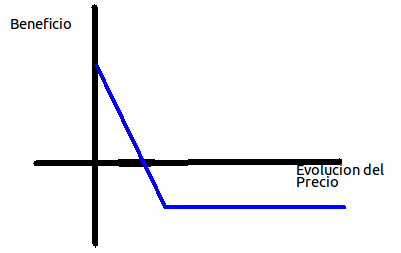
\includegraphics[width=5cm, keepaspectratio]{opcionventacomprador.png}
					\caption{Punto de vista del comprador en t = T}

					\breakcolumn
					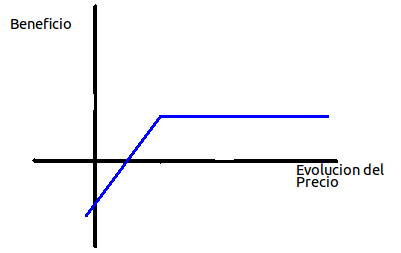
\includegraphics[width=5cm, keepaspectratio]{opcionventavendedor.png}
					\caption{Punto de vista del vendedor en t = T}
					\end{multicols}
				\end{figure}


			\subsubsection{Paridad Put-Call}

				La paridad Put/Call es una relación entre las opciones call, las opciones put y el propio precio del subyacente, de forma que en todo momento debe existir un equilibrio entre los precios. Si se desajusta aparecen oportunidades de arbitraje.

				\subsubsubsection{Opciones europeas sin dividendos}

					Dados los siguientes datos (en el instante de tiempo t):
					\begin{multicols}{2}
					\begin{itemize}
						\item \f{c\sub{t}} precio del call europeo.
						\item \f{X\sub{t}} precio del ejercicio o strike.
						\item \f{r\sub{t}} tipo libre de riesgo.
						\item \f{T} tiempo en el que se tiene derecho a la opción.
						\item \f{p\sub{t}} precio de opción venta europea.
						\item \f{S\sub{t}} precio del subyacente.
					\end{itemize}
					\end{multicols}

					Tenemos que en cualquier instante t, 
						\begin{center} \f{c\sub{t} + X\sub{t}e\pot{-r\sub{t}(T - t)} = p\sub{t} + S\sub{t}} \end{center}

					\n{Derivación}:

					Dadas dos carteras, para \f{t = 0}:
					\begin{itemize}
						\item A compra un call y tiene una cantidad de efectivo \f{Xe\pot{-rT}}, es decir, \f{V\sub{0}(A) = c + Xe\pot{-rT}}.
						\item E compra un put y tiene una acción. \f{V\sub{0}(B) = p + S}.
					\end{itemize}

					En \f{t = T}, tenemos que:
					\begin{itemize} 
						\item A: Si \f{S\sub{T} > X} ejecutamos la opción y obtenemos \f{S\sub{T}}. Si \f{S\sub{T} < X} no ejecutamos la opción y mantenemos X. Por tanto, \f{V\sub{T}(A) = max(X,S\sub{T})}.
						\item E: Si \f{S\sub{T} > X} no ejecutamos la opción de venta S, \f{V\sub{T}(E) = S\sub{T}}. Si \f{S\sub{T} < X} ejecutamos el put, \f{V\sub{T}=X}. Por tanto, \f{V\sub{T}(E) = max(X,S\sub{T})}.
					\end{itemize}

				\subsubsubsection{Opciones americanas sin dividendos}

					Para \n{opciones americanas} tenemos \f{P > p} y \f{C = c} en ausencia de dividendos. Entonces, 
						\begin{center} \f{C - P < S - Xe\pot{-rT}} \end{center}

					\n{Derivación}:
					Dada una cartera F con una opción americana de venta y una acción, y una cartera G con una opción de compra y cantidad de efectivo X:
					\begin{center} \f{S - X < C - P < S - X e\pot{-rT}} \end{center}
				
				\subsubsubsection{Efecto de los dividendos}

					El valor actual de los dividendos de una acción D es un valor deducible durante la vida de una opción cotizable. Los datos X, S, D son valores actuales del mercado, dependen de T.

					Tenemos una cartera H con una opción europea de compra y efectivo de \f{D + Xe\pot{-rT}}. Otra cartera B, con una acción, \f{c > max(S-D-Xe\pot{-rT},0)}.

					Otra cartera E con una opción europea de venta y una acción. Por último, la cartera I con efectivo de \f{D+Xe\pot{-rT}}, con \f{p > max(D+Xe\pot{-rT}-S, 0)}.
					\begin{center} \f{D\sub{0} = de\pot{-rt\sub{0}}} \\ \f{D\sub{T} = d e\pot{r(T-t\sub{0})}} \end{center}

					Usando la cartera E y H tenemos la \n{paridad put-call}: 
					\begin{center} \f{c + D + Xe\pot{-rT} = p + S} \end{center}

					Para una cartera J con opción europea de compra y efectivo de \f{D + X} y otra cartera F con una opción americana de venta y una acción, concluímos:
					\begin{center} \f{S - D - X < C - P < S - Xe\pot{-rT}} \end{center}

	\newpage

\section{Mercados Financieros Finitos}

	\subsection{Situación}

		\begin{itemize}
			\item Consideramos un número finito de tiempos. (\f{0} actualidad, \f{1} una unidad en el futuro).
			\item Tenemos \f{d} posibles activos. \f{S := (S\pot{1},...,S\pot{d})} vector de \n{variables aleatorias} de los elementos del mercado (M). Cada \f{S\sub{t}\pot{i}} es el \n{valor en t del activo \f{S\pot{i}}} es una variable que toma un número finito de valores.
			\item \n{Subyacente sintético}: combinación de dos o más activos.
			\item \f{\Lambda} representa el conjunto de inversores.
			\item \f{F\sub{1} = \sigma(S\sub{1},...,S\sub{d})} es la información del mercado, filtración.
			\item Cada \f{\alpha \in \Lambda} tiene definida en \f{F\sub{1}} una probabilidad \f{P\sub{\alpha}}.
			\item \n{Hipótesis:} \f{\forall \alpha,\beta \in \Lambda}, \f{P\sub{\alpha} \sim P\sub{\beta}}.
		\end{itemize}

	\subsection{Teoría de las carteras}

		\begin{itemize}
			\item \n{Cartera (portafolio)}. Conjunto de todas las posiciones en todos los activos (largos o cortos) que tiene un individuo o institución.
			\item \n{Estrategia}, \f{\varphi}, consiste en la decisión de invertir en tiempo 0 en el activo \f{S\sub{i}} comprando \f{\varphi\sub{i}} unidades y esperar hasta el instante \f{1}. (\n{Modelo de un periodo}).
			\item \n{Valor de la cartera} en \f{t = 0,1} es la variable aleatoria:
			\begin{center} \f{V\sub{t} = \sumatorio{1}{d} \varphi\sub{i}S\sub{t}\pot{i} = \varphi S\sub{t}} \end{center}
			\item \n{Función de precio} \f{\Pi: M \ent \rn{+}} tal que para todo elemento del mercado nos da su precio actual. \f{\Pi(S\pot{i}\sub{1}) = S\sub{0}\pot{i}}.
		\end{itemize}

		\subsubsection{Hipótesis para el mercado y las carteras}

			\begin{itemize}
				\item No existen fricciones en la economía: no hay costes de transacción, no hay impuestos, no hay restricciones a posiciones cortas. 
				\item La competencia es perfecta, los subyacentes disponibles son precio-aceptantes. 
				\item Suponemos subyacentes divisibles.

			\end{itemize}

			\newpage

	\subsubsection{Arbitraje}

		Un \n{arbitraje} es una estrategia de cartera con un número finito de subyacentes donde la posibilidad de ganar sin arriesgar es real. Existirán oportunidad de arbitraje en los siguientes casos. Si existe una estrategia \f{\varphi = (\varphi\sub{1},...,\varphi\sub{d})} tal que:

		\begin{center}
		\begin{tabular}{|c|c|}
			\hline
			Precio & \f{\exists \alpha \in \Lambda} tal que \\ 
			\hline
			\f{\Pi(\varphi S\sub{1}) \leq 0} & \f{P\sub{\alpha}(\varphi S\sub{1} \geq 0) = 1} y \f{P\sub{\alpha}(\varphi S\sub{1} > 0) > 0} \\
			\hline
			\f{\Pi(\varphi S\sub{1})\geq 0} &  \f{P\sub{\alpha}(\varphi S\sub{1} \leq 0) = 1} y \f{P\sub{\alpha}(\varphi S\sub{1} < 0) > 0} \\
			\hline
			\f{\Pi(\varphi S\sub{1}) \neq 0} &  \f{P\sub{\alpha}(\varphi S\sub{1} = 0) = 1} \\
			\hline
			\f{\Pi(\sumatorio{1}{d} \varphi\sub{j}S\pot{j}) \neq \sumatorio{1}{d} \varphi\sub{j} \Pi(S\pot{j})} & \\
			\hline
		\end{tabular}
		\end{center}

		En nuestra economía consideraremos ausencia de arbitrajes.

		\n{Consecuencia}. En ausencia de arbitraje, \f{\forall S \in M} tal que \f{\exists \alpha \in \Lambda} con: 
		\begin{center} \f{P\sub{\alpha}(S\sub{1} \geq 0) = 1} y \f{P\sub{\alpha}(S\sub{1} > 0) > 0} \end{center}
		verifica necesariamente \f{S\sub{0} = \Pi(S\sub{1}) > 0}.

	\subsubsection{Rendimientos relativos}

		Son las variables aleatorias:
		\begin{itemize}
			\item \n{Rendimientos relativos} (rate of return):
				\begin{center} \f{R\sub{i} = \frac{S\sub{1}\pot{i} - S\sub{0}\pot{i}}{S\sub{0}\pot{i}}} \end{center}
			\item \n{Rendimientos} (total return):
				\begin{center} \f{\hat{R}\sub{i} = \frac{S\pot{i}\sub{0}}{S\pot{i}\sub{0}}} \end{center}
		\end{itemize}

		Así tenemos
		\begin{center} \f{V\sub{1} = \sumatorio{1}{d} \varphi\sub{i} S\pot{i}\sub{1} = \sumatorio{1}{d} \varphi\sub{i} S\sub{0}\pot{i}(1+R\sub{i}) = \sumatorio{1}{d} \varphi\sub{i}S\sub{0}\pot{i}\hat{R}\sub{i}} \end{center}

	\subsubsubsection{Teorema de valoración en ausencia de arbitraje}

		El rendimiento (respectivamente para rendimiento relativo) de una cartera es igual a la media ponderada de los rendimientos (resp. rendimientos relativos) de los subyacentes que lo componen.

		\begin{center} \f{\hat{R} = \frac{V\sub{1}}{V\sub{0}} = \frac{\sumatorio{}{} \varphi\sub{i}S\sub{0}\pot{i} \hat{R}\sub{i}}{\sumatorio{}{}\varphi\sub{i}S\pot{i}\sub{0}} = \sumatorio{}{} w\sub{i}\hat{R}\sub{i}} \end{center}

		donde \f{w\sub{i} = \frac{\varphi\sub{i}S\sub{0}\pot{i}}{\sumatorio{}{} \varphi\sub{i}S\sub{0}\pot{i}}} es el peso del i-ésimo activo en la cartera. 

		Análogamente, 
		\begin{center} \f{R = \frac{\Delta \Pi}{\Pi} = \frac{V\sub{1} - V\sub{0}}{V\sub{0}} = \sumatorio{}{} w\sub{i} R\sub{i}} \end{center} 

	\subsection{Prima de riesgo}

		\n{Activo sin riesgo}: \f{S\pot{0}} tal que \f{S\sub{0}\pot{0} = 1}, \f{S\sub{1}\pot{0} = 1 + r\sub{f}} donde \f{r\sub{f}} es su rendimiento, conocido.

		\n{Prima de riesgo} del activo \f{S \in M} con respecto al inversor \f{\alpha \in \Lambda}:
		\begin{center} \f{E\sub{\alpha}[R\sub{S}] - r\sub{f}} \end{center}

		\n{Proposición}. La prima de riesgo de una cartera es la media ponderada de las primas de riesgo de los activos que lo componen. 
		\begin{center} \f{E\sub{\alpha}[R] - r\sub{f} = \sumatorio{}{} w\sub{j}(E\sub{\alpha}[R\sub{j}] - r\sub{j})} \end{center}

	\subsection{Modelo de un periodo}

		\begin{itemize}
			\item Nuestra economía tiene \f{m} posibles estados a vencimiento, con sus probabilidades: \f{\Omega = \{\omega\sub{1},...,\omega\sub{m}\}}, \f{P(\omega\sub{i}) = p\sub{i}}, \f{i = 1,...,m}.
			\item Tenemos \f{N+1} subyacentes, \f{S = (S\pot{0},...,S\pot{N})} y su proceso de precios: \f{S\sub{t} = (S\sub{t}\pot{0},..., S\sub{t}\pot{N})} con \f{t = 0,1}.
			\item Suponemos que los rendimientos de los subyacentes son linealmente independientes. 
			\item \f{N+1 \leq m}, m dimensión del espacio vectorial de las variables aleatorias.
			\item \f{S\pot{0}} es el subyacente sin riesgo, \n{cuenta bancaria}. \\ \f{S\sub{0}\pot{0} = 1} (hipótesis de normalización).
			\\ \f{S\sub{1}\pot{0} > 0}, en general, \f{S\sub{1}\pot{0} \geq 1}.
			\\ Rendimiento del activo sin riesgo \f{r = S\sub{1}\pot{0} - 1} (tipo de interés).
			\item Proceso de \n{precios descontados}:
			\begin{center} \f{\tilde{S}\sub{t} = (\tilde{S}\sub{t}\pot{0},...,\tilde{S}\sub{t}\pot{N})}, \f{\tilde{S}\pot{i}\sub{t} = \frac{S\sub{t}\pot{i}}{S\sub{t}\pot{0}} \forall i, t} \end{center}
			\item \n{Valor descontado} de una cartera:
			\begin{center} \f{\tilde{V}\sub{t}(\varphi) = \frac{V\sub{t}(\varphi)}{S\sub{t}\pot{0}}} \end{center}
			\item El subyacente asociado a los valores descontados actúa como \n{numerario}. (Elegir un numerario es determinar la unidad de trabajo del mercado).
		\end{itemize}

		\subsubsection{Activo contingente y economía completa}

			Un producto financiero \f{X\sub{1}} v.a. en \f{\Omega} es un \n{activo contingente} o \n{replicable} si \f{\exists \varphi} estrategia de cartera tal que \f{X\sub{1} = \varphi S\sub{1}}.

			\n{Economía completa} \f{\sii} todos los activos son replicables.\\
			\n{Economía viable} \f{\sii} no existen oportunidades de arbitraje.

			\n{Proposición}. Si X es replicable \f{X = \varphi S\sub{1}} admite solución. Si la economía es \n{viable} dicha solución es única.

		\subsection{Modelo matricial}

			\n{Modelo matricial}. Tenemos m estados en \f{1} y \f{N+1} subyacentes. Determinar que un activo es replicalbe es resolver un sistema de m ecuaciones con \f{N+1} incógnitas. \f{S\sub{1}} tiene \f{N+1} filas y \f{m} columnas.

		\subsubsection{Resultados}

			\n{Proposición}. Es replicable si los rangos de \f{S\sub{1}} y \f{(X\sub{1}S\sub{1})} son iguales. La economía es completa si el rango de \f{S\sub{1}} es m. Entonces \f{m = N+1}.

			\n{Proposición}. Supongamos que \f{\exists q = (q\sub{1},...,q\sub{m})} \f{q\sub{j} > 0} tal que \f{\forall \varphi} del mercado se verifique: \begin{center} \f{\tilde{V}\sub{0}(\varphi) = \sumatorio{j}{} q\sub{j} \tilde{V}\sub{1}(\varphi)(w\sub{j})} \end{center} Entonces la economía es \n{viable}.

			\n{Proposición}. Bajo la suposición anterior, \f{Q: \Omega \leftarrow \rn{}} tal que \f{Q(w\sub{i}) = q\sub{i} \forall i}. Entonces \f{Q} define una probabilidad en \f{\Omega}, conocida como \n{probabilidad de descuento} o \n{probabilidad de riesgo neutro}.

			\n{Consecuencias}. La condición suficiente de viabilidad se escribe como: 
			\begin{itemize}
				\item \n{Propiedad de martingala con respecto de Q}: \f{\tilde{V}\sub{0}(\varphi) = E\sub{Q}[\tilde{V}\sub{1}(\varphi)]}.
				\item \n{Propiedad de riesgo neutro}. El numerario es la cuenta bancaria y \f{V\sub{0}(\varphi) = \frac{E\sub{Q}[V\sub{1}(\varphi)]}{1+r}}
			\end{itemize}

			\vspace{0.3cm}
			\begin{framed}
			\n{Teorema}. La economía es completa y viable \f{\sii} \f{\exists !} probabilidad de riesgo neutro (o prob. martingala) Q tal que \begin{center} \f{\tilde{V}\sub{0}(\varphi) = E\sub{Q}[\tilde{V}\sub{1}(\varphi)]} \f{\forall \varphi} \end{center}
			\end{framed}
			\vspace{0.3cm}

			\n{Proposición}. Sea P la probabilidad subjetiva de un inversor y Q la probabilidad de riesgo neutro. En una economía \n{viable}: 
			\begin{center} \f{\tilde{S}\sub{0} = E\sub{Q}[\tilde{S}\sub{1}] = E\sub{P}[Z\tilde{S}\sub{1}]} siendo \f{Z(w\sub{j}) = \frac{Q(w\sub{j})}{P(w\sub{j})}} \end{center}

			Esta es la relación que nos define el precio en ausencia de arbitraje con una probabilidad subjetiva. Z es la \n{densidad o vector de estados de los precios}.

			\begin{center} Si \f{Q \sim P} \f{\ent Z = \frac{dQ}{dP}} \end{center}

			\n{Proposición}. Sea \f{S\pot{n}} subyacente tal que \f{S\sub{1}\pot{n}(w\sub{j}) \neq 0} \f{\forall w\sub{j}\in \Omega}. Entonces \f{S\pot{n}} es un numerario.

			\n{Teorema}. Sea una economía \n{completa y viable}. Sean \f{S\pot{n}} y \f{S\pot{m}} dos numerarios, \f{Q\sub{n},Q\sub{m}} las probabilideades martingalas asociadas. Entonces:
			\begin{center} \f{S\sub{0}\pot{n} E\sub{Q\sub{n}}[S\sub{1}\pot{i}/S\sub{i}\pot{n}] = S\sub{0}\pot{m} E\sub{Q\sub{m}}[S\sub{1}\pot{i}/S\sub{i}\pot{m}]} \f{\forall i = 0,...,N} \end{center}

		\subsubsection{Activos de Arrow-Debreu}

			Sea una economía completa y viable. Los \n{activos de Arrow-Debreu} \f{A\sub{T}\pot{i}} para \f{i = 1,...,m} se definen como: 
			\begin{center} \f{A\sub{T}\pot{i}(w\sub{j}) = \delta\sub{ij}} para \f{j = 1,...,m} \end{center}

			\n{Proposición}. Sean \f{A\sub{0}\pot{i}} el valor en \f{0} de los activos Arrow-Debreu. Entonces para cualquier subyacente:
			\begin{center} \f{S\sub{0} = \sumatorio{1}{m} S\sub{T}(w\sub{i})A\sub{0}\pot{i}} \end{center}

			\n{Proposición}. Sea S un activo numerario. Entonces, la probabilidad martingala asociada a S es:
			\begin{center} \f{Q\sub{S}(w\sub{i}) = \frac{S\sub{T}(w\sub{i}) A\sub{0}\pot{i}}{S\sub{0}}} \end{center}

			Esto permite calcular los \f{A\sub{0}\pot{i}}, la probabilidad martingala Q, las densidades entre probabilidades martingalas: 
			\begin{center} \f{Q\sub{n}}, \f{Q\sub{m}} probabilidades \f{Z\sub{nm}(w\sub{j}) = \frac{Q\sub{n}(w\sub{j})}{Q\sub{m}(w\sub{j})}} \end{center}

	\newpage

	\section{Modelo binomial}

		El \n{modelo binomial} es un modelo discreto que permite observar el comportamiento de un activo (por ejemplo, acción) a través del tiempo. El precio de la acción puede comportarse de \n{dos} formas: subir o bajar en cada unidad de tiempo. Denotamos:
		\begin{itemize}
			\item \n{Precios} (consideramos modelo multiplicativo). En particular, para el modelo de un paso tenemos \f{S\sub{0}}, precio actual de la acción, \f{S\sub{1} = a S\sub{0}}, precio de la acción en el caso de subida y \f{S\sub{1} = b S\sub{0}}, precio de la acción en el caso de bajada. Consideramos (teóricamente) que \boldf{a > b} y \boldf{a b = 1}. En general, tenemos \f{N+1} precios, dados por: 
			\begin{center} \f{ S\sub{n+1} = \left\{
				\begin{aligned} 
					& aS\sub{n} \text{   alza} \\
					& bS\sub{n} \text{   baja} \\
				\end{aligned}
				}
			\end{center}
			\item \n{Probabilidades}. \f{p\sub{\alpha}} de subida y \f{1-p\sub{\alpha}} de bajada. Se considera para un inversor \f{\alpha \in \Lambda}.

				\begin{figure}[h!]
					\begin{center}
					\includegraphics[width=8.5cm, height=6.5cm]{binomial.png}
					\end{center}
				\end{figure}
			
			\item \f{\omega} camino aleatorio del árbol. Hay \f{2\pot{N}} trayectorias posibles, \f{\Omega = \{\omega\sub{1},...,\omega\sub{2\pot{N}}\}}
			\item \n{Número de subidas} hasta n, \f{Z\sub{n}(\omega)}, es una variable aleatoria que sigue una distribución binomial \f{B(n,p\sub{\alpha})}. \f{Z\sub{n}(\omega) = \sumatorio{i = 1}{n} Z\sub{i}} donde \f{Z\sub{i} = \left\{ \begin{aligned} 1 \text{ si hay subida en } t\sub{i}  \\ 0 \text{  si hay bajada en } t\sub{i} \end{aligned}}
			\item \f{S\sub{n}(\omega)} para \f{n = 0,...,N}, precio del camino. \begin{center} \boldf{S\sub{n}(\omega) = S\sub{0} a\pot{Z\sub{n}(\omega)} b\pot{n-Z\sub{n}(\omega)}} \end{center}
			\item La probabilidad de cada camino es: 
			\begin{center} \f{P\sub{\alpha}(\omega) = p\sub{\alpha}\pot{Z\sub{N}(\omega)}(1-p\sub{\alpha})\pot{N-Z\sub{N}(\omega)}} \hspace{0.3cm} \f{\forall \omega \in \Omega} \end{center}
			\item \n{Filtración}. \f{F\sub{n} = \sigma(S\sub{1},S\sub{2},...,S\sub{n})}. Es una sigma-álgebra del conjunto de posibles trayectorias, \f{\Omega}, (conjunto de subconjuntos de \f{\Omega}, cerrado por complementación, por uniones arbitrarias e intersecciones finitas). Representa también los precios posibles para los caminos aleatorios de un árbol de n pasos. Cumplen que \f{F\sub{i} \subseteq F\sub{i+1} \forall i = 0,...,N}. Por ejemplo, \f{F\sub{0} = \{\emptyset, \Omega\}}. \\ \f{F\sub{1} = \{\emptyset, \Omega, A, B\}} donde \f{A} denota el suceso \f{\{S\sub{1} = a S\sub{0}\}} y \f{B} denota \f{\{S\sub{1} = bS\sub{0}\}}. \\ \f{F\sub{2} = \{\emptyset, \Omega, A, B, AA, BB, AB, BA, BB\}}.
			
		\end{itemize}

		\begin{multicols}{2}
		\begin{itemize}
			\item Los inversores coinciden en N-periodos y fechas de transacción.
			\item Se pueden fraccionar los activos.
			\item No se pagan dividendos, no hay costes de transacción ni impuestos.
			\item Se permiten descubiertos ilimitados en \f{t}.
		\end{itemize}
		\end{multicols}

		\subsection{Resultados}

			\begin{itemize}
				\item Un \n{activo replicable} es una variable aleatoria \f{F\sub{n}}-medible.
				\item La dinámica del \n{activo sin riesgo} está caracterizada por su rendimiento. \begin{center} \f{S\sub{n}\pot{0} = (1+r)S\sub{n-1}\pot{0}} \f{\forall n = 1,...,N}, \f{S\sub{0}\pot{0} = 1}\end{center}
				\item La \n{probabilidad de riesgo neutro} en un periodo es: 
				\begin{center} \f{q = \frac{1+r-b}{a-b}}, \hspace{0.3cm} \f{1-q = \frac{a -1-r}{a-b}} \end{center}
				\item La probabilidad de riesgo neutro del modelo binomial es:
				\begin{center} \f{Q(\omega) = q\pot{Z\sub{N}(\omega)} (1-q)\pot{N-Z\sub{N}(\omega)}} \f{\forall \omega \in \Omega} \end{center}
				\item Los precios descontados son una martingala.
				\begin{center} \f{\frac{S\sub{m}}{(1+r)\pot{m}} = E\sub{Q}[\frac{S\sub{n}}{(1+r)\pot{n}}|F\sub{m}]} \f{\forall 0 \leq m < n \leq N} \end{center}
				\item En particular, el \n{precio de un activo}:
				\begin{center} \f{S\sub{0} = E\sub{Q}[\frac{S\sub{N}}{(1+r)\pot{N}}]} \end{center}
				\item \n{Teorema}. La economía descrita por el modelo binomial es \n{completa}. %(Todos los activos son replicables).
			\end{itemize}
		
		\subsection{Martingala}

			Sea \f{(\Omega, F, P)} un espacio de probabilidad finito, \f{F\sub{0}, F\sub{1}, ..., F\sub{N}} álgebras de subconjuntos de F tal que: \f{F\sub{0} \subseteq F\sub{1} \subseteq ... \subseteq F\sub{N}} = F}, es filtración de F.

			Una sucesión de variables aleatorias \f{S\sub{1},...,S\sub{n}} sobre \f{(\Omega, F, P)} se llama \n{martingala} respecto a \f{F\sub{0},F\sub{1},...,F\sub{N}} si \f{S\sub{n}} es \f{F\sub{n}}-medible y \f{E[X\sub{n+1}| F\sub{n}] = S\sub{n}}.

		\subsection{Carteras autofinanciadas}

			El inversor rebalancea su cartera en función de la economía en ese momento. Cada \n{estrategia} es un proceso estocástico: \boldf{\varphi\sub{n}(\omega) = (\varphi\pot{0}\sub{n}(\omega), \varphi\pot{1}\sub{n}(\omega))}, donde \f{\varphi\pot{i}\sub{n}(\omega)} es el número de unidades del activo \f{i} durante \f{(n,n+1]}. La redistribución viene dada por: \boldf{\varphi\sub{n+1} S\sub{n+1} = \varphi\sub{n}S\sub{n+1}}.

			Dada una estrategia \f{\varphi}, \f{V\sub{n}(\varphi)} es el valor de la cartera en \f{n}, \f{n \leq N} y verifica

			\begin{center} \f{V\sub{n+1}(\varphi) - V\sub{n}(\varphi) = \varphi\sub{n} (S\sub{n+1} - S\sub{n})} \hspace{0.3cm} \f{V\sub{n+1}(\varphi) = V\sub{0}(\varphi) + \sumatorio{j = 0}{n} \varphi\sub{j} (S\sub{j+1} - S\sub{j})} \end{center}

			Sin arbitraje, el \n{valor de una cartera} cuyo flujo en N es \f{\varphi(S\sub{N})} viene dado por: \begin{center} \boldf{V\sub{0} = \frac{1}{(1+r)\pot{N}} E\sub{Q}[\varphi(S\sub{N})]} \end{center}
 		

		\subsection{Valor de una opción de compra europea}

			Una opción europea c de strike K con \f{aS\sub{0} < K < bS\sub{0}} tiene como precio y estrategia:

			\begin{itemize}
				\item Para el modelo de \f{1} paso:
				\begin{center} \f{c\sub{0} = \frac{(aS\sub{0} - K)(1+r-b)}{(1+r)(a-b)}} y \f{\varphi\pot{1}\sub{0} = \frac{aS\sub{0}-K}{(a-b)S\sub{0}}} \end{center}

				\item En general, dado una opción con flujo final \f{X = (S\sub{N} - K)\pot{+}}, \f{X(\omega) = max(S\sub{N}(\omega) \menos K, 0)}, el valor es:
				\begin{center} \f{c\sub{0} = V\sub{0} = \frac{1}{(1+r)\pot{N}} E\sub{Q}[(S\sub{N}-K)\pot{+}] =} \\ \f{= \frac{1}{(1+r)\pot{N}} \sumatorio{n=0}{N} \left( \begin{matrix} N \\ n \end{matrix} \right) q\pot{n} (1-q)\pot{N-n} (S\sub{0}a\pot{n}b\pot{N-n} - K)\pot{+}} \end{center}
			\end{itemize}

			La ausencia de arbitraje nos da la \n{paridad call-put}: 
			\begin{center} \f{c\sub{n} - p\sub{n} = S\sub{n} - K(1+r)\pot{n-N}} \end{center}
			También podemos calcular el valor de un put, a partir del call.

			\subsubsection{Derivación de las fórmulas del modelo de \f{1} paso (cartera réplica)}

				Vamos a valorar una opción de compra europea formando una \n{cartera réplica} a partir del derivado y un activo libre de riesgo (cuenta bancaria), es decir, creando un activo gemelo que genere los mismos flujos de caja que el activo a valorar.

				La cartera se compone de \f{h} acciones y de un préstamo de \f{B} euros a un tipo de interés libre de riesgo \f{r\sub{f}} (no tiene riesgo porque en todo momento habrá dinero para devolver el préstamo). Por tanto, dentro de un período los flujos de caja de dicha cartera son, dados los siguientes precios:

				\begin{center}
				\begin{tabular}{|c|c|c|c|}
					\hline
					& Actual & Subida & Bajada\\
					\hline
					Acción & \f{S\sub{0}} & \f{S\sub{a} = aS\sub{0}} & \f{S\sub{b} = bS\sub{0}}\\
					\hline
					Call & \f{c\sub{0}} & \f{c\sub{a} = max(S\sub{a} - K, 0)} & \f{c\sub{b} = max(S\sub{b} - K, 0)} \\
					\hline
					Flujos cartera & \f{S\sub{0}h - B} & \f{S\sub{a}h - (1+r\sub{f})B } & \f{S\sub{b}h - (1+r\sub{f})B} \\
					\hline
				\end{tabular}
				\end{center}

				Para que no haya \n{oportunidades de arbitraje}, el modelo considera: \f{c\sub{0} = S\sub{0}h - B}. Tenemos: \\ \f{c\sub{a} = S\sub{a} h - (1+r\sub{f})B} \hspace{0.3cm} \f{c\sub{b} = S\sub{b} h - (1+r\sub{f})B} \end{center}

				Restando ambas ecuaciones se obtiene el ratio de cobertura, \f{h = \frac{c\sub{u} - c\sub{d}}{S\sub{0}} (a - b)}. \\ Tenemos que \f{B = \frac{S\sub{a}h - c\sub{a}}{1+r\sub{f}}}.

				Sustituyendo los valores anteriores en la ecuación de \f{c\sub{0}} y considerando las \n{probabilidades neutrales de riesgo}: \f{q = \frac{1+r-b}{a-b}}, \f{1-q = \frac{a -1-r}{a-b}}, se llega a que el precio teórico de la opción de compra es igual al valor actual de la media ponderada de los flujos de caja que proporciona:
				\begin{center} \f{c = \frac{c\sub{a}q + c\sub{b}(1-q)}{1+r\sub{f}}} \end{center}

				\n{Observación}. Las \n{\cur{probabilidades} neutrales al riesgo} no son probabilidades formalmente, son los precios tiempo-estado de los posibles estados (subida-bajada) multiplicados por \f{1+r\sub{f}}. Pero ambas suman \f{1}, son positivas y se emplean para estimar el rendimiento esperado de un activo con riesgo que hacen que la prima de riesgo desaparezca.

		\subsection{Arbitraje}
				
			El modelo binomial es libre de arbitraje (la economía es viable) si \f{0 < p\sub{\alpha} < 1} y \boldf{b < 1 + r < a}.


		\subsection{Ajustes del árbol a datos del mercado}

			Sea \f{T} tiempo hasta vencimiento, \f{\Delta t} tiempo entre dos nodos y \f{r\sub{c}} el tipo libre de riesgo anual (con composición continua). Tenemos:
			\begin{center} \f{e\pot{r\sub{c}} = 1 + r \ent r \approx r\sub{c}\Delta t} \end{center}

			La \n{probabilidad de riesgo neutro} verifica: \f{q = \frac{e\pot{r\sub{c}\Delta t} - b}{a-b}}.

			La \n{volatilidad} de un activo, \f{\sigma}, verifica que, para un \f{\Delta t} pequeño, la desviación típica de sus rendimientos es \f{\sigma\sqrt{\Delta t}}.

			El marco natural para el rendimiento relativo \f{\hat{R} = S\sub{n+1}/S\sub{n}}. Se verifica: 
				\begin{center} \f{e\pot{r\sub{c}\Delta t} = E\sub{Q}[\hat{R}] = aq + b(1-q)} \\ \f{\sigma\pot{2} \Delta t = V\sub{Q}[\hat{R}] = a\pot{2}q + b\pot{2}(1-q) - e\pot{2r\sub{c}\Delta t}} \end{center}

			Tenemos dos ecuaciones con tres incógnitas (\f{a,b,q}). Existen distintas aproximaciones:
			\begin{itemize}
				\item \n{Cox-Russ-Rubinstein}. Para \f{ab = 1}, \f{a = e\pot{\sigma\sqrt{\Delta t}}}, \f{b = e\pot{-\sigma \sqrt{\Delta t}}}.
				\item \n{Jarrod-Rudd}, \f{q = 0.5}. \f{a = e\pot{(r\sub{c}-\frac{\sigma\pot{2}}{2}) \Delta t} e\pot{\sigma \sqrt{\Delta t}}}, \f{b = e\pot{(r\sub{c}-\frac{\sigma\pot{2}}{2}) \Delta t} e\pot{-\sigma \sqrt{\Delta t}}}.
				\item \n{Tian}. Añadimos la ecuación de los momentos de orden \f{3} que hace coincidir el modelo binomial con el modelo continuo: \f{a\pot{3}q + b\pot{3}(1-q) = e\pot{3r\sub{c}\Delta t} e\pot{3\sigma\pot{2} \Delta t}}.
				Entonces, 
				\begin{center} \f{q = \frac{(e\pot{r\sub{c}\Delta t} - b)}{(a-b)}} \\ \f{a = \frac{e\pot{(r\sub{c}+\sigma\pot{2})\Delta t}}{2} [e\pot{\sigma\pot{2} \Delta t} + 1 + \sqrt{e\pot{2\sigma\pot{2}\Delta t} + 2 e\pot{\sigma\pot{2} \Delta t} - 3}]} \\
				\f{b = \frac{e\pot{(r\sub{c}+\sigma\pot{2})\Delta t}}{2} [e\pot{\sigma\pot{2} \Delta t} + 1 - \sqrt{e\pot{2\sigma\pot{2}\Delta t} + 2 e\pot{\sigma\pot{2} \Delta t} - 3}]} \end{center}
			\end{itemize}

		\subsection{Fórmula de Cox-Rubinstein}

				Valor de un call es: 
				\begin{center} \f{c\sub{0} = S\sub{0} \phi(n\sub{0},N,q') - \frac{K}{(1+r)\pot{N}}\phi(n\sub{0},N,q)} \end{center}

				donde \begin{center} \f{\varphi(n\sub{0},N,q) = P(X\geq n\sub{0})} donde \f{X \sim B(N,q)} \end{center}

				y \f{n\sub{t} = [\frac{ln(K/(Sb\pot{N}))}{ln(a/b)}] + 1} y \f{q' = \frac{aq}{1+r}}.


		
\printindex

\end{document}
